=\renewcommand{\theequation}{\theenumi}
\begin{enumerate}[label=\arabic*.,ref=\thesubsection.\theenumi]
\numberwithin{equation}{enumi}
\item P(A) be the prbability of concentration of sulpher

\begin{table}[!ht]
\begin{tabular}{ |c|c| } 
	\hline
	\textbf{concentration of sulphur} &\textbf{friquency}\\
	\hline
	0.01 &2\\ 
	0.02 &1\\ 
	0.03 &1\\ 
	0.04 &2\\ 
	0.05 &2\\ 
	0.06 &2\\ 
	0.07 &3\\
	0.08 &4\\ 
	0.09 &2\\ 
	0.10 &1\\ 
	0.11 &2\\ 
	0.12 &1\\ 
	0.13 &1\\ 
	0.16 &1\\ 
	0.17 &1\\ 
	0.18 &2\\ 
	0.20 &1\\ 
	0.22 &1\\   
	\hline
\end{tabular}	
	\caption{This is a table template}
	\label{tab:template}
\end{table}
\begin{align}
p\left(A\right) &= \frac{1+1+1}{30}
\\
&= 0.1
\end{align}
codes for the above equation can be get from here
\begin{lstlisting}
codes/prob/prob10.py
\end{lstlisting}
\begin{figure}[!ht]
	\centering
	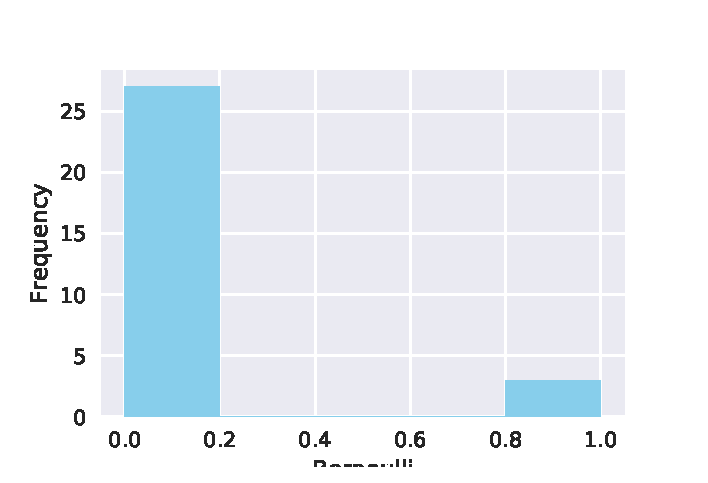
\includegraphics[width=\columnwidth]{./figures/prob/prob10.eps}
	\caption{probability of $SO_2$ 0.12 to 0.16 }
	\label{fig:bt9}
	\begin{lstlisting}
	figs/prob/prob10.py
	\end{lstlisting}
\end{figure}
\end{enumerate}